%! Author = User
%! Date = 13.09.2023

% Preamble
\documentclass[a4paper,10pt,twocolumn]{article}

% Packages 
\usepackage[utf8]{inputenc}  %man kann Sonderzeiche wie ü,ö usw direkt eingeben
\usepackage{amsmath}           %macht
\usepackage{amsfonts}          %       Mathe
\usepackage{amssymb}           %              mächtiger
\usepackage{graphicx}          %erlaubt Graphiken einzubinden (.eps für dvi und ps sowie .jpg für pdf)
\usepackage[T1]{fontenc}       %Zeichenbelegung der verwendeten Schrift
\usepackage{ae}                %macht schöneres ß
\usepackage{typearea}
\usepackage{amstex}
\usepackage{siunitx}
\usepackage{hyperref}	         %ermöglicht änderung des Seitenspiegels


\usepackage{amsmath}
\usepackage{tikz}
\usepackage{pgfplots}

\newcommand{\alphaNoError}{(4.047 \pm 0.036)}
\newcommand{\betaNoError}{(-4.73 \pm 0.29) \cdot 10^{-3}}
\newcommand{\halfTimeNoError}{(146.5 \pm 9.1)\ s}
\newcommand{\alphaGauss}{(4.04 \pm 0.10)}
\newcommand{\betaGauss}{(-4.62 \pm 0.95) \cdot 10^{-3}}
\newcommand{\halfTimeGauss}{(150 \pm 31)\ s}
\newcommand{\alphaPoisson}{(4.05 \pm 0.10)}
\newcommand{\betaPoisson}{(-4.75 \pm 0.95) \cdot 10^{-3}}
\newcommand{\halfTimePoisson}{(146 \pm 29)\ s}
\newcommand{\symN}{\delta N}



\pagestyle{scrheadings}        %sagt Koma-Skript, dass selbstdefiniers Kopfzeilen verwendet werden
\typearea{16}                  %stellt Seitenspiegel ein
\columnsep25pt								 %definiert Breite zwischen den zwei Spalten von \twocolumns

\renewcommand{\pnumfont}{%     %ändert die Schriftart der Seitennummerierung
    \normalfont\rmfamily\slshape}  %ändert die Schriftart der Seitennummerierung 



\begin{document}
    \twocolumn[{\csname @twocolumnfalse\endcsname                %erlaubt "Abstrakt" über beide Spalten
    \titlehead{                                                  %Kopfzeile
        \begin{tabular*}{\textwidth}[]{@{\extracolsep{\fill}}lr}   %Kopfzeile
            Tutor: ? & \today\\                          %Kopfzeile - Betreuer
        \end{tabular*}                                             %Kopfzeile
    }
    \title{Experimental methods for examining properties of classical light with microwaves and using bragg reflection to examin cirstal structur}  %Titel der Versuchs
    \author{Salahudin Smailagić and Thomas Karb}                     %Namen der Studenten
    \date{}                                                         %benötigt um automatisches Datum auszuschalten
    \maketitle                                                      %erzeugt Titelseite
    \vspace{-5ex}                                                   %verringert Abstand zur Überschrift
    \begin{abstract}                                                %Beginn des Abstracts
        We used experiments with microwaves to show the wave character of light.
        Basic methods are used to test our devices.
        Via inteference and stationary waves we determined the wavelenght.
        Furthermore we verify the properties polarisation and total reflection.
        And we demonstrate the method of bragg diffraction with a cristel model.
        \\
        Measuerement made: 21. September 2023\\       %Datum ändern!
        Submitted: 26. September 2023                %Datum ändern!
        \\
        \\
    \end{abstract}
    }]
    \section{Introduction}
    To study wave-properties of light we use microwaves.
    They have a large wave lenght in the cm-range.
    Effects like interference and tunneling occur on a macroscopic scale, which makes it easy to show them
    in an experiment.
    Because all properties showed here with microwaves apply also for light in the visible spectrum, you can use 
    reuse our results, but on a different scale of length.
    \section{Experimental setup}
    \subsection{Emitter}
    A Gunn diode was used to create the microwaves in our experiments. 
    It has a horn antenna for focusing the light.
    We measured the angle-intensity-relation and made a basic gauss-fit to get a rough estimate of the light dispersion (cf.~\ref{fig:AngleDispersion}).
    The full-width-half-maximum of the used emitter is
    \begin{align*}
        fwhm = \AngleDispersionGaussFWHM
    \end{align*}

    \figAngleDispersion{Angle dispersion of the Gunn diode used in our setup.
    We fit a gauss curve to get an approximation of the variance. 
    $fwhm = \AngleDispersionGaussFWHM$}


    \subsection{Lens}
    For the experiments with bragg reflection and tunnel effect we need parallel light rays.
    We used a wax lens for focusing the emitted microwaves.
    To determine the focal length, the lens was placed away from the emitting diode.
    The effective object (emitter) distance after~\cite{pasco} in our setup was $g = \ObjectDistance$
    Then by varying the receiver positions the intensity was measured as shown in figure ~\ref{fig:imageDistance}. 
    Because the wavelength is in the cm range, the diameter of the resulting airy disk is also in the cm range.
    This means there is no distance were the object (emitter) is completely focused as you would expect from geometric optics.
    So to access the image distance we made a gauss-fit over the intensity distribution and used the maximum of the fit as
    reference. 
    
    \figimageDistance{We measure the signal depending on the reciever-lens distance $b$.
    The intensity fluctuates since a stationary wave overlaps.
    We apply a gauss-fit to get the maximum image distance.
    This can be used to calculate the focal length after the lens formula ~\eqref{eq:LensFormula}}
    
    Here the image distance is 
    \begin{align*}
        b = \ImageDistance
    \end{align*}

    Now we can calculate the focal length after the lens formula
    \begin{align}
        \label{eq:LensFormula}
        \frac{1}{f} = \frac{1}{b} + \frac{1}{g}
    \end{align}
    We have determined the focal length of the lens in our setup as:
    \begin{align*}
        f = \FocalLength
    \end{align*}
    \section{Wavelength measurement}
    It is important to know the wavelength of the light for the subsequent experiments.
    The wavelength by the manufacturer of the diode is
    \begin{align*}
        \lambda = \OfficialWaveLength
    \end{align*}
    To verify this we used two setups.
    \subsection{Stationary wave}
    For the first approach we create stationary waves.
    We position a mirror opposite of the emitter in a distance of $1m$.
    Then we move the receiver between mirror and diode and count the nodes of the resulting standing wave.
    We then measure the distance around 40 nodes and can calculate the wavelength:
    \begin{align*}
        \lambda = \StandingWavesWaveLength
    \end{align*}
    \subsection{Michelson interferometer}
    As the second approach we use an interferometer.
    The emitted light is split by a fiberboard as semi-transparent mirror in two perpendicular rays.
    They are then reflected by two metal sheets and reunited again by the fiberboard. 
    In the resulting ray interferes constructive or destructive depending on the difference between the two optical paths .
    We move the position of one mirror and after seeing 15 maxima and minima on the detector we read the changed
    path length.
    With our setup we have determined the wavelength as:
    \begin{align*}
        \lambda = \InterferometerWaveLength
    \end{align*}
    \begin{figure}[htbp]
        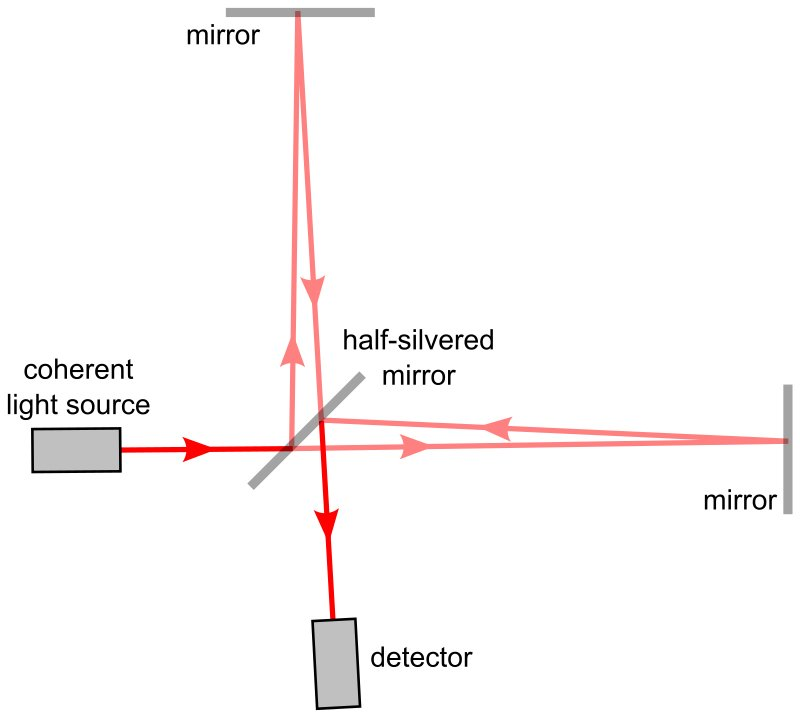
\includegraphics[width=0.9\linewidth]{Interferometer}
        \center
        \caption{By varing the optical path length of the rays you see constructive or destructive interference on the
        detector. This depends on the wavelength of the ligth, which enables you to measure it.
        Graphic from~\cite{imageMichelsonInterferometerWiki}}
        \label{fig:Interferometer}
    \end{figure}
    \section{Polarisation}
    The Gunn diode with the horn antenna in our setup emits vertical polarized light.
    Also the receiver detects in default configuration only vertical polarized light.
    This can be easily shown by rotating the receiver about $ 90\degree$.
    Now no signal is being detected.
    If you then insert a linear polarisation filter in a $ 45\degree$ angle you will detect a signal.
    This follows because the vertical polarized E-field is projected on the polarisation filter.
    For the polarisation filter a simple metal grid was used with 22 lattice bars.

    As a quantitative assertion we arranged the receiver and emitter in vertical position and rotated the polarisation
    filter in an $ 180\degree $-arc and measured the angle-intensity distribution.
    Following Malus's law~\cite{gerth} the intensity after the filter is:
    \begin{align}
        I = I_0 \cos^2(\phi)
    \end{align}
    Since the metal grid and the receiver act as two polarisation filter our signal should follow the formula:
    \begin{align}
        \label{eq:cos4}
        I = I_0 \cos^4( \phi )
    \end{align}
    If we compare the theoretical function to the measured data as in ~\ref{fig:Polarisation} we see a strong deviation.
    This is probably due to the low number of lattice bars, which makes the polarisation filter not ideal.
    \figPolarisation{Transmitted intensity through a polarisation filter. 
    Though the shape of the curve fits, there is a strong deviation from the theory by Malus ~\eqref{eq:cos4}}
    
    \section{Total inner reflection and tunnel effect}
    An important property of light which we were able to show, is total reflection and evanescent waves.
    For the experiment we emitted microwaves on a paraffin wax prism. 
    On the $45\degree$ paraffin-air boundary the rays are totally reflected and we detect them in an $90\degree$ rotated
    angle. 
    After the paraffin-air boundary an evanescent wave is formed.
    Its intensity declines exponentially.
    \begin{align}
        I \propto e^{\frac{-2x}{s}} 
    \end{align}
    Here $x$ is the perpendicular distance and $s$ is the declination rate which depends on the wavelength, 
    the angle of reflection and the refractive index.

    You can detect the evanescent wave by a adding a second prism after the $ 45\degree$ boundary parallel to the first one
    in the distance $x$.
    Now analogous to the quantenmechanical tunnel effect\cite{gerth} the light can propagate through the air gap and a signal can be
    detected.
    We have measured the reflected and transmitted microwaves for different gap sizes $x$ and then applied an exponential 
    fit as you can see in~\ref{fig:TotalReflection}

    \figTotalReflection{We measure the transmitted and reflected signal at a double prism.
    The transmitted signal declines exponentially. This can be explained by the tunnel effect.}

    \section{Bragg Reflection}
    If you have monochromatic waves with a wavelength around the atomic scale (x-ray, neutrons or electrons) you can
    determine the lattice constant d of a cubic cristal via bragg diffraction. 
    In Bragg's model the cristal is a set of discrete planes where waves are reflected.
    If the waves have the correct wavelength and hit the planes in the correct angle the reflected waves interfere 
    constructively and you see a bragg peak as a result~\cite{gerth}.
    
    The cristal planes can be indexed via the parameters $h,\,k,\,l$.
    For the angle $\Theta$ where a break peak occurs the following relation applies:
    \begin{align}
        \label{eq:BraggAngle}
        \frac{d}{\sqrt{h^2+k^2+l^2}} = \frac{\lambda}{2 \sin(\Theta)}
    \end{align}
    
    To demonstrate the principle we use a basic cristal model, consisting of metal bars arranged in a grid structure.
    For examining real crystals it would require electromagnetic waves with much smaller wavelengths.
    We realize the experiment by placing the emitter in the focal point of the wax lens, so the cristal is hit by
    parallel light rays.
    The cristal model is then rotated about $\Theta$ and the detector about $2\Theta$ to actualize the Bragg condition.
    
    We have done two measurement series: For the plane-orientation $h = 1,\,k = 0,\,l = 0$ and for $h = 1,\,k = 1,\\l = 0$ as 
    you can see in figure~\ref{fig:BraggReflectionOneZeroZero} and figure~\ref{fig:BraggReflectionOneOneZero}.
    If we use equation~\eqref{eq:BraggAngle} to calculate the lattice constant from our measurement series, we get:
    \begin{align*}
        d_{100} = \CristalconstantOneZeroZero \\
        d_{110} = \CristalconstantOneOneZero
    \end{align*}
    
    \figBraggReflectionOneZeroZero{Bragg diffraction on the 100-plane of a cubic lattice model.
    A peak was detected at the first bragg-maxima}
    \figBraggReflectionOneOneZero{Bragg diffraction on the 110-plane of a cubic lattice model.
    Here the bragg-peak occurs at a greater angle compared to the 100-palne}

    \section{Waveguide}
    
    Lastly we examined a simple waveguide for microwaves.
    We used a basic metal tube.
    The waves are being reflected in its interior and thus guided by the tube.
    We placed the emitter at one end of the tube and the receiver at the other.
    A signal is being detected.
    If you put a plug on the one end, no signal is being blocked.
    This proves the waves are guided inside of the tube and not on its surface.
    Also the tube preserves the polarisation of the emitted light.
    This was shown by simply rotating the receiver, since it only detects v-polarized light.

    \section{Summary}
    
    At first we tested our experimental setup.
    The Gunn diode has a gaussian angle-intensity distribution with a variance $fwdh = \AngleDispersionGaussFWHM$.
    To focus the microwaves we used a wax lens with a focal length $f = \FocalLength$.
    Then we used two approaches to measure the wavelength. 
    Via stationary waves we get a wavelength $\lambda = \StandingWavesWaveLength$.
    The michelson interferometer produces a similar result $\lambda = \InterferometerWaveLength $.
    We could show the polarization of the emitted light and at least qualitatively verify Malus' law. 
    The effect of total reflection and tunnel effect was demonstrated by using a double prism.
    The intensity of the evanescent waves declines exponentially.
    We used a cristal model to show the method of bragg diffraction.
    The lattice constant was determined to $d_{100} = \CristalconstantOneZeroZero$.
    At last we used a metal tube as waveguide.
    We demonstrated qualitatively it preserves the polarisation of the guided light.
    
    
    %FF: Angabe der verwendeten Literatur mit Quellennachweis.
    \begin{thebibliography}{}    %so wird das Literaturverzeichnis erstellt
        \bibitem{instr} Physikalisches Grundpraktikum, Universitüt Würzburg, Modul C1, Versuch 42, Versuche mit Mikrowellen - Kristallinterferenzen mit Mikrowellen, 2021
        \bibitem{gerth} Meschede, Dieter, Gerthsen Physik, 25. Auflage, Springer-Verlag, Berlin, 2015
        \bibitem{codata} P. J. Mohr, D. B. Newell, and B. N. Taylor: \grqq CODATA
        recommended values of the fundamental physical constants: 2014\grqq , Rev. Mod. Phys.
        88, 035009 (2016))
        %\bibitem{miller} \url{https://de.wikipedia.org/wiki/Datei:Miller_Indizes_Ebenen.png}, zuletzt aufgerufen am 14.09.2021
        \bibitem{pasco} Pasco Microwave Optics System (WA-9314C) Instruction Manual
        %\bibitem{missing} \url{https://en.wikipedia.org/wiki/Transverse_mode}, zuletzt aufgerufen am 8.10.2021
        \bibitem{imageMichelsonInterferometerWiki} \url{https://en.wikipedia.org/wiki/Michelson_interferometer#/media/File:Michelson_interferometer_with_labels.svg}, last visit 23.09.23
    \end{thebibliography}
    
\end{document}